\chapter{My First Content Chapter}
\label{chapterlabel2}

Often lots of citations here (and elsewhere), e.g. \cite{Rey:D} or \cite[Theorem 2.3]{PriorNOP70}.   Bibtex can help with this, but is not essential. If you want pictures, try

\begin{center}
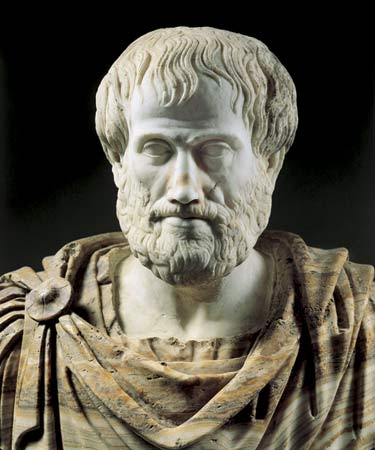
\includegraphics[scale=.5]{aristotle.jpg}
\end{center}
You can use 
\begin{itemize}
\item lists
\item like this
\end{itemize}
or numbered
\begin{enumerate}
\item like this,
\item or this
\end{enumerate}
but don't overdo it.

% This just dumps some pseudolatin in so you can see some text in place.
\blindtext
